
%(BEGIN_QUESTION)
% Copyright 2010, Tony R. Kuphaldt, released under the Creative Commons Attribution License (v 1.0)
% This means you may do almost anything with this work of mine, so long as you give me proper credit

This schematic diagram shows a pneumatic sensing mechanism (based loosely on the Bettis DeltaMatic pipeline valve shutoff system) designed to take action when the gas pressure inside of a process vessel begins to change at a sufficient {\it rate} over time:

$$\includegraphics[width=15.5cm]{i04429x01.eps}$$

Analyze this diagram, then answer the following questions:

\begin{itemize}
\item{} Does this mechanism activate (i.e. switch out of its ``normal'' state) when the process pressure's rate of change {\it rises} quickly over time, {\it falls} quickly over time, or rapidly changes in {\it either} direction?
\vskip 10pt 
\item{} Identify what would have to be altered in this mechanism to make the previous answer different (i.e. make the mechanism respond to a different direction of process pressure change).
\vskip 10pt 
\item{} Identify the direction of air flow through the line leading to the ``pneumatic control device'' when the process pressure is not changing at all.
\vskip 10pt 
\item{} Identify one component that would have to be altered in this mechanism to make it {\it less sensitive} to rates of process gas pressure change over time, and also identify how that component would have to be altered (e.g. size, shape, etc.).
\end{itemize}

\vfil 

\underbar{file i04429}
\eject
%(END_QUESTION)





%(BEGIN_ANSWER)

\begin{itemize}
\item{} This mechanism activates when the process pressure's rate of change {\bf rises} quickly over time.
\vskip 10pt 
\item{} To switch the direction of change, both the check valve and the spool valve's return spring would have to be reversed in direction.
\vskip 10pt 
\item{} Identify the direction of air flow through the line leading to the ``pneumatic control device'' when the process pressure is not changing at all: {\bf air flowing in from the pneumatic control device}.
\vskip 10pt 
\item{} Identify one component that would have to be altered in this mechanism to make it {\it less sensitive} to rates of process gas pressure change over time, and precisely how that component would have to be altered (e.g. size, shape, etc.): either {\bf enlarge the restriction}, {\bf shrink the capacity tank}, and/or {\bf replace the spool valve spring with one that is ``stiffer''}.
\end{itemize}


%(END_ANSWER)





%(BEGIN_NOTES)


%INDEX% Mechanics, fluid power systems: analysis of pneumatic rate-of-change detection system

%(END_NOTES)


